\chapter{Marco Teórico}

\section{Arquitectura de Software y Patrón Modelo-Vista-Controlador (MVC)}
En la ingeniería de software moderna, la separación de responsabilidades constituye un principio medular para garantizar la escalabilidad, mantenibilidad y modularidad de las aplicaciones web \cite{pressman2010, sommerville2011}. El patrón arquitectónico Modelo-Vista-Controlador (MVC), introducido originalmente por Trygve Reenskaug y consolidado en la arquitectura de aplicaciones empresariales por Martin Fowler \cite{fowler_patterns}, desacopla el sistema en tres capas interconectadas:

\begin{itemize}
    \item \textbf{Modelo (Model):} Representa la capa lógica del dominio del negocio y gobierna las reglas de acceso, validación y persistencia de datos. En el ecosistema Laravel, los modelos extienden la clase \texttt{Illuminate\textbackslash Database\textbackslash Eloquent\textbackslash Model}, implementando el patrón \textit{Active Record} \cite{laravel_doc}.
    \item \textbf{Vista (View):} Constituye la capa de presentación que se encarga de estructurar y desplegar la información al usuario final. Se implementa mediante el motor de plantillas Blade, permitiendo la composición de interfaces limpias, reutilizables y con soporte de componentes jerárquicos.
    \item \textbf{Controlador (Controller):} Actúa como el intermediario orquestador que intercepta las peticiones HTTP despachadas por el sistema de enrutamiento, invoca la lógica de los modelos correspondientes y retorna la respuesta adecuada (vistas renderizadas o respuestas JSON estructuradas).
\end{itemize}

\section{Entorno de Ejecución Backend: PHP 8.4 y Framework Laravel 11}
El backend de la plataforma se cimenta sobre la versión \textbf{PHP 8.4}, la cual introduce mejoras significativas en el compilador JIT (Just-In-Time), soporte nativo de tipos estrictos, promoción de propiedades en constructores y tipado de retorno explícito \cite{php_manual}. Estas características incrementan la seguridad en tiempo de compilación/ejecución y reducen errores comunes de tipado.

Sobre este entorno opera el framework \textbf{Laravel 11.x}, que destaca por su robusto contenedor de inyección de dependencias, sistema de eventos, cola de tareas en segundo plano y una capa de abstracción de base de datos de alto nivel \cite{laravel_doc}. La arquitectura de rutas de Laravel permite definir filtros declarativos mediante \textit{Middleware}, asegurando la verificación de sesiones y roles antes de transferir el control a los controladores.

\section{Persistencia de Datos Relacional y Eloquent ORM}
La gestión de inventario multisede y bienes coleccionables exige un motor de base de datos relacional que cumpla rigurosamente con las propiedades ACID (Atomicidad, Consistencia, Aislamiento y Durabilidad) \cite{sommerville2011}. Para tal fin se emplea \textbf{MariaDB}, utilizando el motor transaccional InnoDB \cite{mariadb_foundation}.

\begin{figure}[htbp]
    \centering
    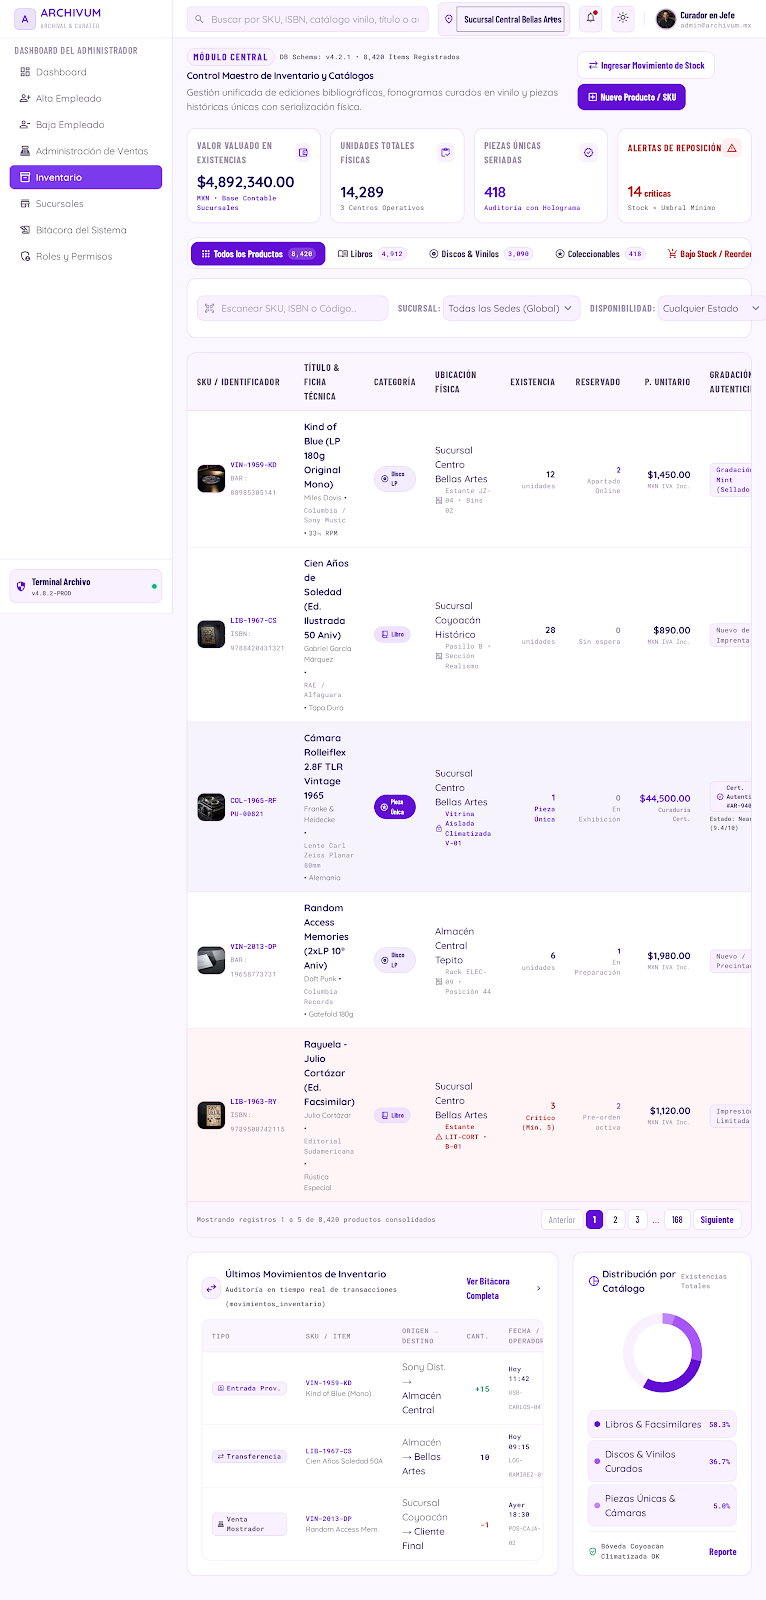
\includegraphics[width=0.82\textwidth, height=8.5cm, keepaspectratio]{imagenes/inventario_unificado.png}
    \caption{Visualización y control unificado de inventario y existencias patrimoniales.}
    \label{fig:teoria_inventario_unificado}
\end{figure}

El mapeador objeto-relacional (ORM) Eloquent simplifica la interacción con la base de datos permitiendo definir relaciones complejas:
\begin{itemize}
    \item \textbf{Relaciones de Uno a Muchos (\texttt{hasMany} / \texttt{belongsTo}):} Aplicadas entre categorías y productos, así como entre sucursales y sus registros específicos de inventario.
    \item \textbf{Relaciones de Muchos a Muchos (\texttt{belongsToMany}):} Utilizadas en pedidos y productos a través de tablas pivote con metadatos asociados (cantidad, precio unitario de venta y estado de entrega).
    \item \textbf{Migraciones y Seeders:} Permiten versionar la estructura de la base de datos en código PHP reproducible y poblar registros semilla iniciales para pruebas controladas.
\end{itemize}

\section{Virtualización Ligera y Orquestación con Docker}
El despliegue de soluciones web corporativas demanda independencia del sistema operativo anfitrión. \textbf{Docker} proporciona un mecanismo de virtualización a nivel de sistema operativo mediante contenedores Linux ligeros, compartiendo el kernel pero aislando por completo los procesos, librerías y dependencias de la aplicación \cite{docker_overview}.

Mediante la herramienta de orquestación \textbf{Docker Compose}, el entorno de \say{Archivum} se organiza en una topología de tres servicios coordinados sobre una red privada virtual:
\begin{enumerate}
    \item \textbf{Servidor Web Nginx:} Procesa peticiones HTTP/HTTPS concurrentes, sirve archivos estáticos optimizados y actúa como proxy inverso hacia el backend \cite{nginx_admin}.
    \item \textbf{Contenedor PHP-FPM:} Aloja el intérprete de PHP 8.4 y la aplicación Laravel, ejecutando el código fuente montado en volúmenes compartidos.
    \item \textbf{Servidor MariaDB:} Provee almacenamiento persistente montado sobre un volumen Docker dedicado, protegiendo los datos ante reinicios de contenedor.
\end{enumerate}

\section{Diseño Frontend, Reactividad y Visualización Analítica}
Para garantizar una experiencia de usuario interactiva y fluida sin incurrir en la sobrecarga computacional de un entorno Single Page Application (SPA) monolítico, se adoptó un enfoque híbrido y ligero:
\begin{itemize}
    \item \textbf{Tailwind CSS:} Framework CSS orientado a utilidades que permite estructurar interfaces modernas con un sistema de tokens de diseño uniforme (espaciado, paleta amatista, tipografía y soporte nativo de tema oscuro/claro) \cite{tailwind_docs}.
    \item \textbf{Alpine.js:} Provee reactividad declarativa para componentes interactivos del cliente (modales, menús desplegables, carritos flotantes) directamente en el marcado HTML de las vistas Blade, manteniendo un footprint inferior a 15 KB \cite{alpinejs_docs}.
    \item \textbf{Chart.js:} Biblioteca gráfica basada en el elemento \texttt{<canvas>} de HTML5, utilizada en el panel administrativo para generar gráficas de líneas y áreas degradadas con renderizado adaptativo según el tema activo \cite{chartjs_org}.
\end{itemize}

\section{Seguridad Web y Control de Acceso Basado en Roles (RBAC)}
La seguridad de la información es un requerimiento no funcional de máxima prioridad en la plataforma. Siguiendo las directrices del proyecto \textit{OWASP Top 10} \cite{owasp_top10}, se implementaron los siguientes mecanismos de defensa:
\begin{itemize}
    \item \textbf{Mitigación de Inyección SQL:} El ORM Eloquent y el constructor de consultas utilizan internamente vinculación de parámetros PDO (\textit{prepared statements}), impidiendo la inyección de sentencias SQL maliciosas.
    \item \textbf{Protección contra Cross-Site Request Forgery (CSRF):} Cada formulario generado por Blade incluye un token criptográfico único verificado por el middleware \texttt{VerifyCsrfToken}.
    \item \textbf{Control de Acceso Basado en Roles (RBAC):} Diferenciación estricta de privilegios entre los roles \texttt{Administrador}, \texttt{Encargado de Sucursal} y \texttt{Cliente}, impidiendo que usuarios sin autorización accedan a rutas operativas o de auditoría financiera.
    \item \textbf{Cifrado de Contraseñas:} Empleo del algoritmo de hash seguro \texttt{Bcrypt} con factores de trabajo dinámicos para el resguardo de credenciales de usuario.
\end{itemize}
